\documentclass{article}
\usepackage{graphicx}
\usepackage{amsmath}
% avoid new line with a tab
\usepackage[parfill]{parskip}
\usepackage{hyperref}
\graphicspath{ {./figures/} }

\title{COMP.SEC.220 Security Protocol\footnote{github -- \url{https://github.com/ancuongnguyen07/SecurityProtocol}}}
\author{Cuong Nguyen - LAB 2}
\date{06/09/2022}

\begin{document}
    
\maketitle

\section*{Exercise 1}
%
I chose the CBC mode of AES symmetic block cipher because its simplicity --- one of
classic modes. But in terms of authentication, we should consider modern modes such as
CCM, EAX, GCM, SIV, and OCB.\\

Plaintext: \textbf{Welcome to the Security Protocols course}\\
Ciphertext (base64):\\
\textbf{wJR/a8AR0ymG/7HR556SIViaHa4owzbkRE+hANVjlGsShMd+KyYoO1I+wptGppo1}

\begin{figure}[hpt]
    \centering
    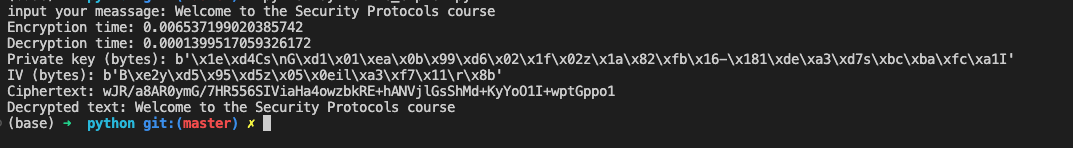
\includegraphics[width=140mm, height=30mm]{aes.png}
    \caption{AES-256-CBC-mode encrytion-decrytion time}
    \label{fig:aes-cbc}
\end{figure}

As you can see in the figure\ref*{fig:aes-cbc}, the decryption takes a shorter time than
the encryption process, faster than 60 times in this case. In the above case, my script
generated a random secret key and an initial vector.\\

\begin{figure}[hpt]
    \centering
    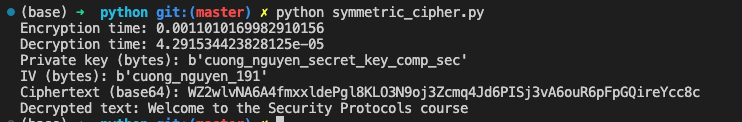
\includegraphics[width=140mm, height=30mm]{aes_chosen_key.png}
    \caption{AES-256-CBC-mode with chosen a private key and an initial vector}
    \label{fig:aes-cbc-chosen}
\end{figure}

Without generating IV and private key, the encryption-decryption process took a shorter
period to finish.

\section*{Exercise 2}
%
\subsection*{RSA}
%
It worth noting that the process of decryption-signing is much slower than those of
encryption-verification (signing and verification used in digital signatures).
In this exercise, I used PKCS#1 OAEp is an asymmetric cipher based on RSA and the
OAEP padding, detailed description \href{https://tools.ietf.org/html/rfc8017}{here}.

\begin{figure}[hpt]
    \centering
    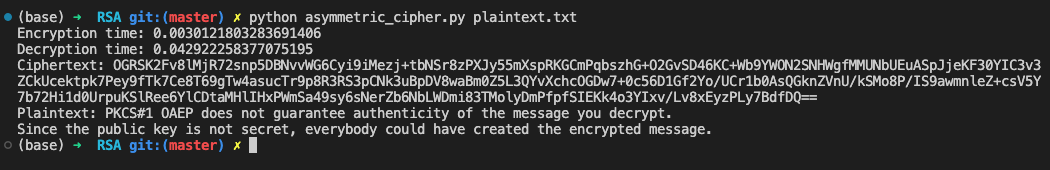
\includegraphics[width=140mm, height=40mm]{rsa.png}
    \caption{RSA-based encrytion-decrytion time}
    \label{fig:rsa}
\end{figure}

\subsection*{Eliptic Curve}
%
\begin{figure}[hpt]
    \centering
    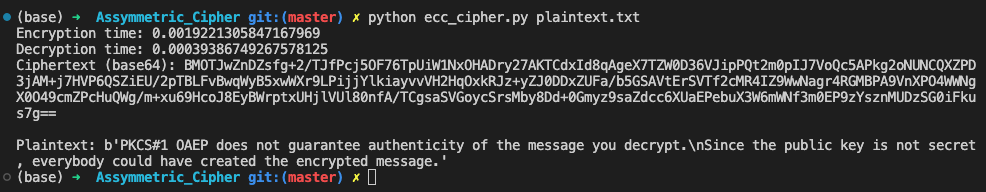
\includegraphics[width=140mm, height=50mm]{ecc.png}
    \caption{EC-based encrytion-decrytion time}
    \label{fig:ec}
\end{figure}

As you can see in the figure~\ref{fig:ec}, the encryption time is much longer than 
the decryption time, constrasting to the RSA scheme

\section*{Exercise 3}
%
To verify the integrity of the specific file, we need to compute the hash digest of the
recieved file, then compare it to the hash digest which was sent along with the file.
If they matches each other, so the file was not modified, otherwise the file was intervened.

\begin{figure}
    \centering
    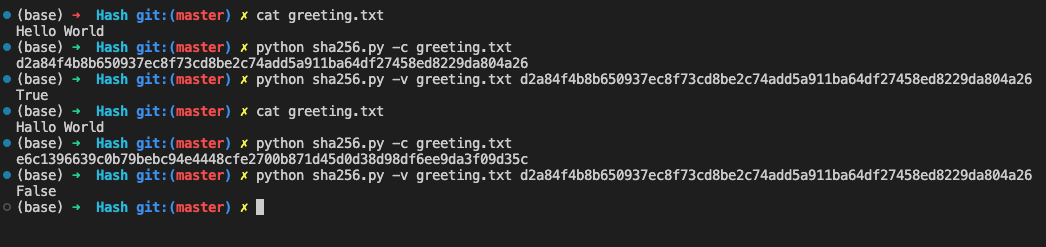
\includegraphics[width=140mm, height=50mm]{sha256.png}
    \caption{SHA256 verification-cumputation}
    \label{fig:sha256}
\end{figure}

As you can see in the figure~\ref{fig:sha256}, when I just changed one letter ``e'' to ``a'', the
generated hash digest was change totally (not partially one letter), showing that hash function
has the property of diffusion.

\end{document}